\chapter{MHD spectroscopy of a solar atmosphere} \label{ch: solar_atmosphere}

\graphicspath{{06-solar_atmosphere/figures/}}

\begin{chapterquote}[Jean-Luc Picard][Star Trek TNG: `Attached']
  There is a way out of every box, a solution to every puzzle; it's just a matter of finding it.
\end{chapterquote}

\usespublishedwork{
  Most of this Chapter was published in ``Magnetohydrodynamic Spectroscopy of a Non-Adiabatic Solar Atmosphere'', 2021, Solar Physics, 296, 9 \citep{claes2021}. N. Claes performed the simulations, did the analysis, and wrote the manuscript; R. Keppens contributed to the revision of the paper.
}

In this Chapter we perform a detailed, high-resolution spectroscopic study of the solar atmosphere, using the newly developed {\legolas} code to calculate the full spectrum with corresponding eigenfunctions of equilibrium configurations that are based on fully realistic solar atmosphere models. Physical effects include gravity, optically thin radiative losses, and thermal conduction. We will give special attention to thermal instabilities, known to be responsible for the formation of solar prominences, and present a new outlook on the thermal and slow continua and how they behave in different chromospheric and coronal regions. We will show that thermal instabilities are unavoidable in the solar atmosphere models used in this Chapters, and that there exist entire regions where both the thermal, slow, and fast modes all have unstable wave mode solutions. Special regions are encountered where the slow and thermal continua become purely imaginary, merging on the imaginary axis. These studies mark the first time a detailed eigenspectrum analysis has been done on a self-consistent solar atmosphere model; all spectra discussed in this Chapter illustrate clearly that thermal instabilities (both discrete and continuum modes) and magnetothermal overstable propagating modes are ubiquitous throughout the solar atmosphere, and may well be responsible for much of the observed fine-structuring and multi-thermal dynamics.

\section{Introduction}
The solar atmosphere shows a myriad of thermodynamically fascinating features, from solar prominences to coronal rain, over plumes, jets, etc. Extensive research on all these features has been done over the past decades, and currently nonlinear MHD simulations are starting to resolve aspects at resolutions rivalling upcoming and future solar telescopes.
A fully self-consistent solar flare model achieving resolutions of 50 km was recently shown in \citet{ruan2020}, while \citet{jenkins2021} focused more on the physical processes driving prominence formation, increasing the resolution even further down to 5 km. In realistic solar atmospheric evolutions many linear waves and instabilities can be at play and interact with one another, implying that modern nonlinear simulations can benefit greatly from the full knowledge of all linear instabilities and eigenoscillations of a given configuration. Some early attempts were made by for example \citet{nye1976}, who discussed an analytical model of the solar atmosphere based on an isothermal slab, where certain mode types of the magnetised atmosphere could be computed analytically in ideal MHD. \citet{vanderlinden1991} did some pioneering work in linear MHD including non-adiabatic effects, hinting at the role of magnetothermal modes in prominence fine-structuring, but since then further research into this topic has stalled.

While fully nonlinear, quasi-realistic numerical simulations can accurately model a plethora of physical phenomena, one can not underestimate the importance of linear MHD. Looking at the saturation of a single unstable mode in the context of prominence formation is one thing, but a \emph{detailed} knowledge of which particular mode among a myriad of unstable eigenmodes is responsible for the evolution can only be obtained through a detailed and careful spectroscopic analysis of a given state. As mentioned before, this has been realised by \citet{demaerel2016}, where they showed -- in ideal MHD, including self-gravity -- that spectral theory actually governs the stability of single-fluid evolving time-dependent plasmas, at every point during their nonlinear evolution. Knowing all MHD modes of (possibly coupled mode types) in a magnetised solar atmosphere, and how they modify as a result of including relevant non-adiabatic effects, is thus a clear necessity in studying solar prominences and their intriguing fine structure. In this Chapter we set out to do exactly this for a realistic solar atmosphere model, in which we include all relevant physical effects important for thermal instability and prominence formation -- that is, external gravity, radiative cooling, and anisotropic thermal conduction. To date there exists no detailed MHD spectroscopic treatment of such a self-consistent model.

There are in fact a wide range of existing interesting studies regarding thermal instabilities and waves in non-adiabatic solar atmosphere-like settings. \citet{zavershinskii2019} demonstrated the formation of slow magneto-acoustic wave trains due to linear dispersion associated with heating-cooling imbalance, while recently \citet{duckenfield2021} looked at slow-mode damping rates in solar coronal conditions under the influence of thermal imbalance and showed that these may be intricately linked. \citet{ledentsov2021} on the other hand looked at thermal instability in preflare current layers including viscosity and the effect that a longitudinal magnetic field has on spatial stabilisation. Studies like these are quite limited however, in the sense that they have to drastically reduce their mathematical models to either homogeneous background conditions in 2D or 3D setups, or to 1D treatments along magnetic field lines in order to be able to derive a dispersion relation or to make the problem analytically tractable.

Armed with our new {\legolas} code we are now able to do a complete eigenspectrum analysis of a fully realistic solar atmosphere model, where we adopt the widely used semi-empirical temperature profile proposed by \citet{avrett2008}, thereby including all aforementioned physical effects. We pay special attention to both the thermal and slow continua, both of which play a very important role in the (in)stability of a given equilibrium configuration. The intricate structure of the thermal, slow, and Alfv\'en continua, and the way that the many discrete modes organise themselves in (coupled) thermal, slow, Alfv\'en and fast wave sequences, is demonstrated here for the first time, giving us a linear ``preview'' of how nonlinear simulations should develop as a result of interacting instabilities. The main advantage of using {\legolas} here is that we are not bound by the same limitations as previous works, in the sense that we do not need any dispersion relation or continuous background profiles in order to calculate growth rates, meaning we can go far beyond that which has already been done in existing literature in our treatment of the solar atmosphere.

In Section \ref{sec: analytical_work} we first revisit the analytical work done by \citet{nye1976} and complement this by looking at non-parallel propagation and the inclusion of non-adiabatic effects, something that was impossible in the original analytical treatment. This will serve as a stepping stone to Section \ref{sec: solar_atmosphere}, where we finally look at a fully realistic solar atmosphere model and perform a detailed spectroscopic analysis with special attention to thermal instabilities. Herein we demonstrate that thermal instability is ubiquitously present in both the solar chromosphere and corona, and provide a fresh outlook on mode behaviour in these regions. In the solar chromosphere, we will show that it becomes possible for the slow continua to merge with the imaginary axis, indicating ``upwards'' and ``downwards'' branches that in turn may become unstable if the conditions are right.


\section{Revisiting analytical models} \label{sec: analytical_work}
We first revisit a solar atmospheric model described by \citet{nye1976}, who considered an isothermal atmosphere with a horizontal magnetic field independent of height and an exponentially decreasing density profile in a uniform gravitational field. This particular setup results in a constant sound speed and density scale height, which, combined with a wave vector parallel to the magnetic field, makes it analytically tractable. The equilibrium background is given in normalised units by
\begin{equation} \label{eq: nye-thomas}
  \begin{gathered}
    \soundspeed^2 = \gamma T_0,
    \qquad
    H = \frac{T_0}{g} = \text{const.}, \\
    \rho_0(x) = \rho_{00}\exp(-x/H),
    \qquad
    B_{0z} = \sqrt{\gamma \rho_{00}T_0 \beta^2} = \text{const.},
  \end{gathered}
\end{equation}
where $H$ denotes the density scale height, $\rho_{00}$ is taken equal to one, and $\beta^2 = c_\text{A0}^2/\soundspeed^2$ is a dimensionless parameter (not to be confused with the plasma beta), defined as the ratio between the Alfv\'en velocity at $x = 0$ and the (constant) sound speed. Furthermore solar gravity is assumed, hence the dimensional value for $g = 274$ m s$^{-2}$ ($\approx$ 1.66 in normalised units). In our setup we take a reference scale height of one and use that to constrain the background temperature. \citet{nye1976} then proceeded in deriving a dispersion relation for waves with a wavenumber $k_z$ purely aligned with the constant horizontal magnetic field, which was then evaluated for various values of $Hk_z$ and $\beta^2$. We on the other hand can plug in the equilibrium configuration defined in Equation \eqref{eq: nye-thomas} in {\legolas} which will return the full eigenvalue spectrum with all eigenfunctions. It should be noted that the original work only considers modes in the fast sequence, while in our full spectrum calculations also the slow and Alfv\'en sequences are present. Also, the analytical work assumes an infinite atmosphere with exponential vanishing eigenfunctions bounded by a slid wall at the lower boundary, while here we have a finite slab with solid wall boundaries on both sides. We therefore take the slabsize sufficiently large (about 15 scale heights) to approximate an infinite atmosphere. All runs in this Section are performed using a resolution of 250 grid points and unit normalisations taken as 1 MK, 10 Gauss, and 50 Mm for the unit temperature, unit magnetic field, and unit length, respectively.


\subsection{Purely parallel propagation} \label{ss: parallel_propagation}
\begin{figure}[t]
  \centering
  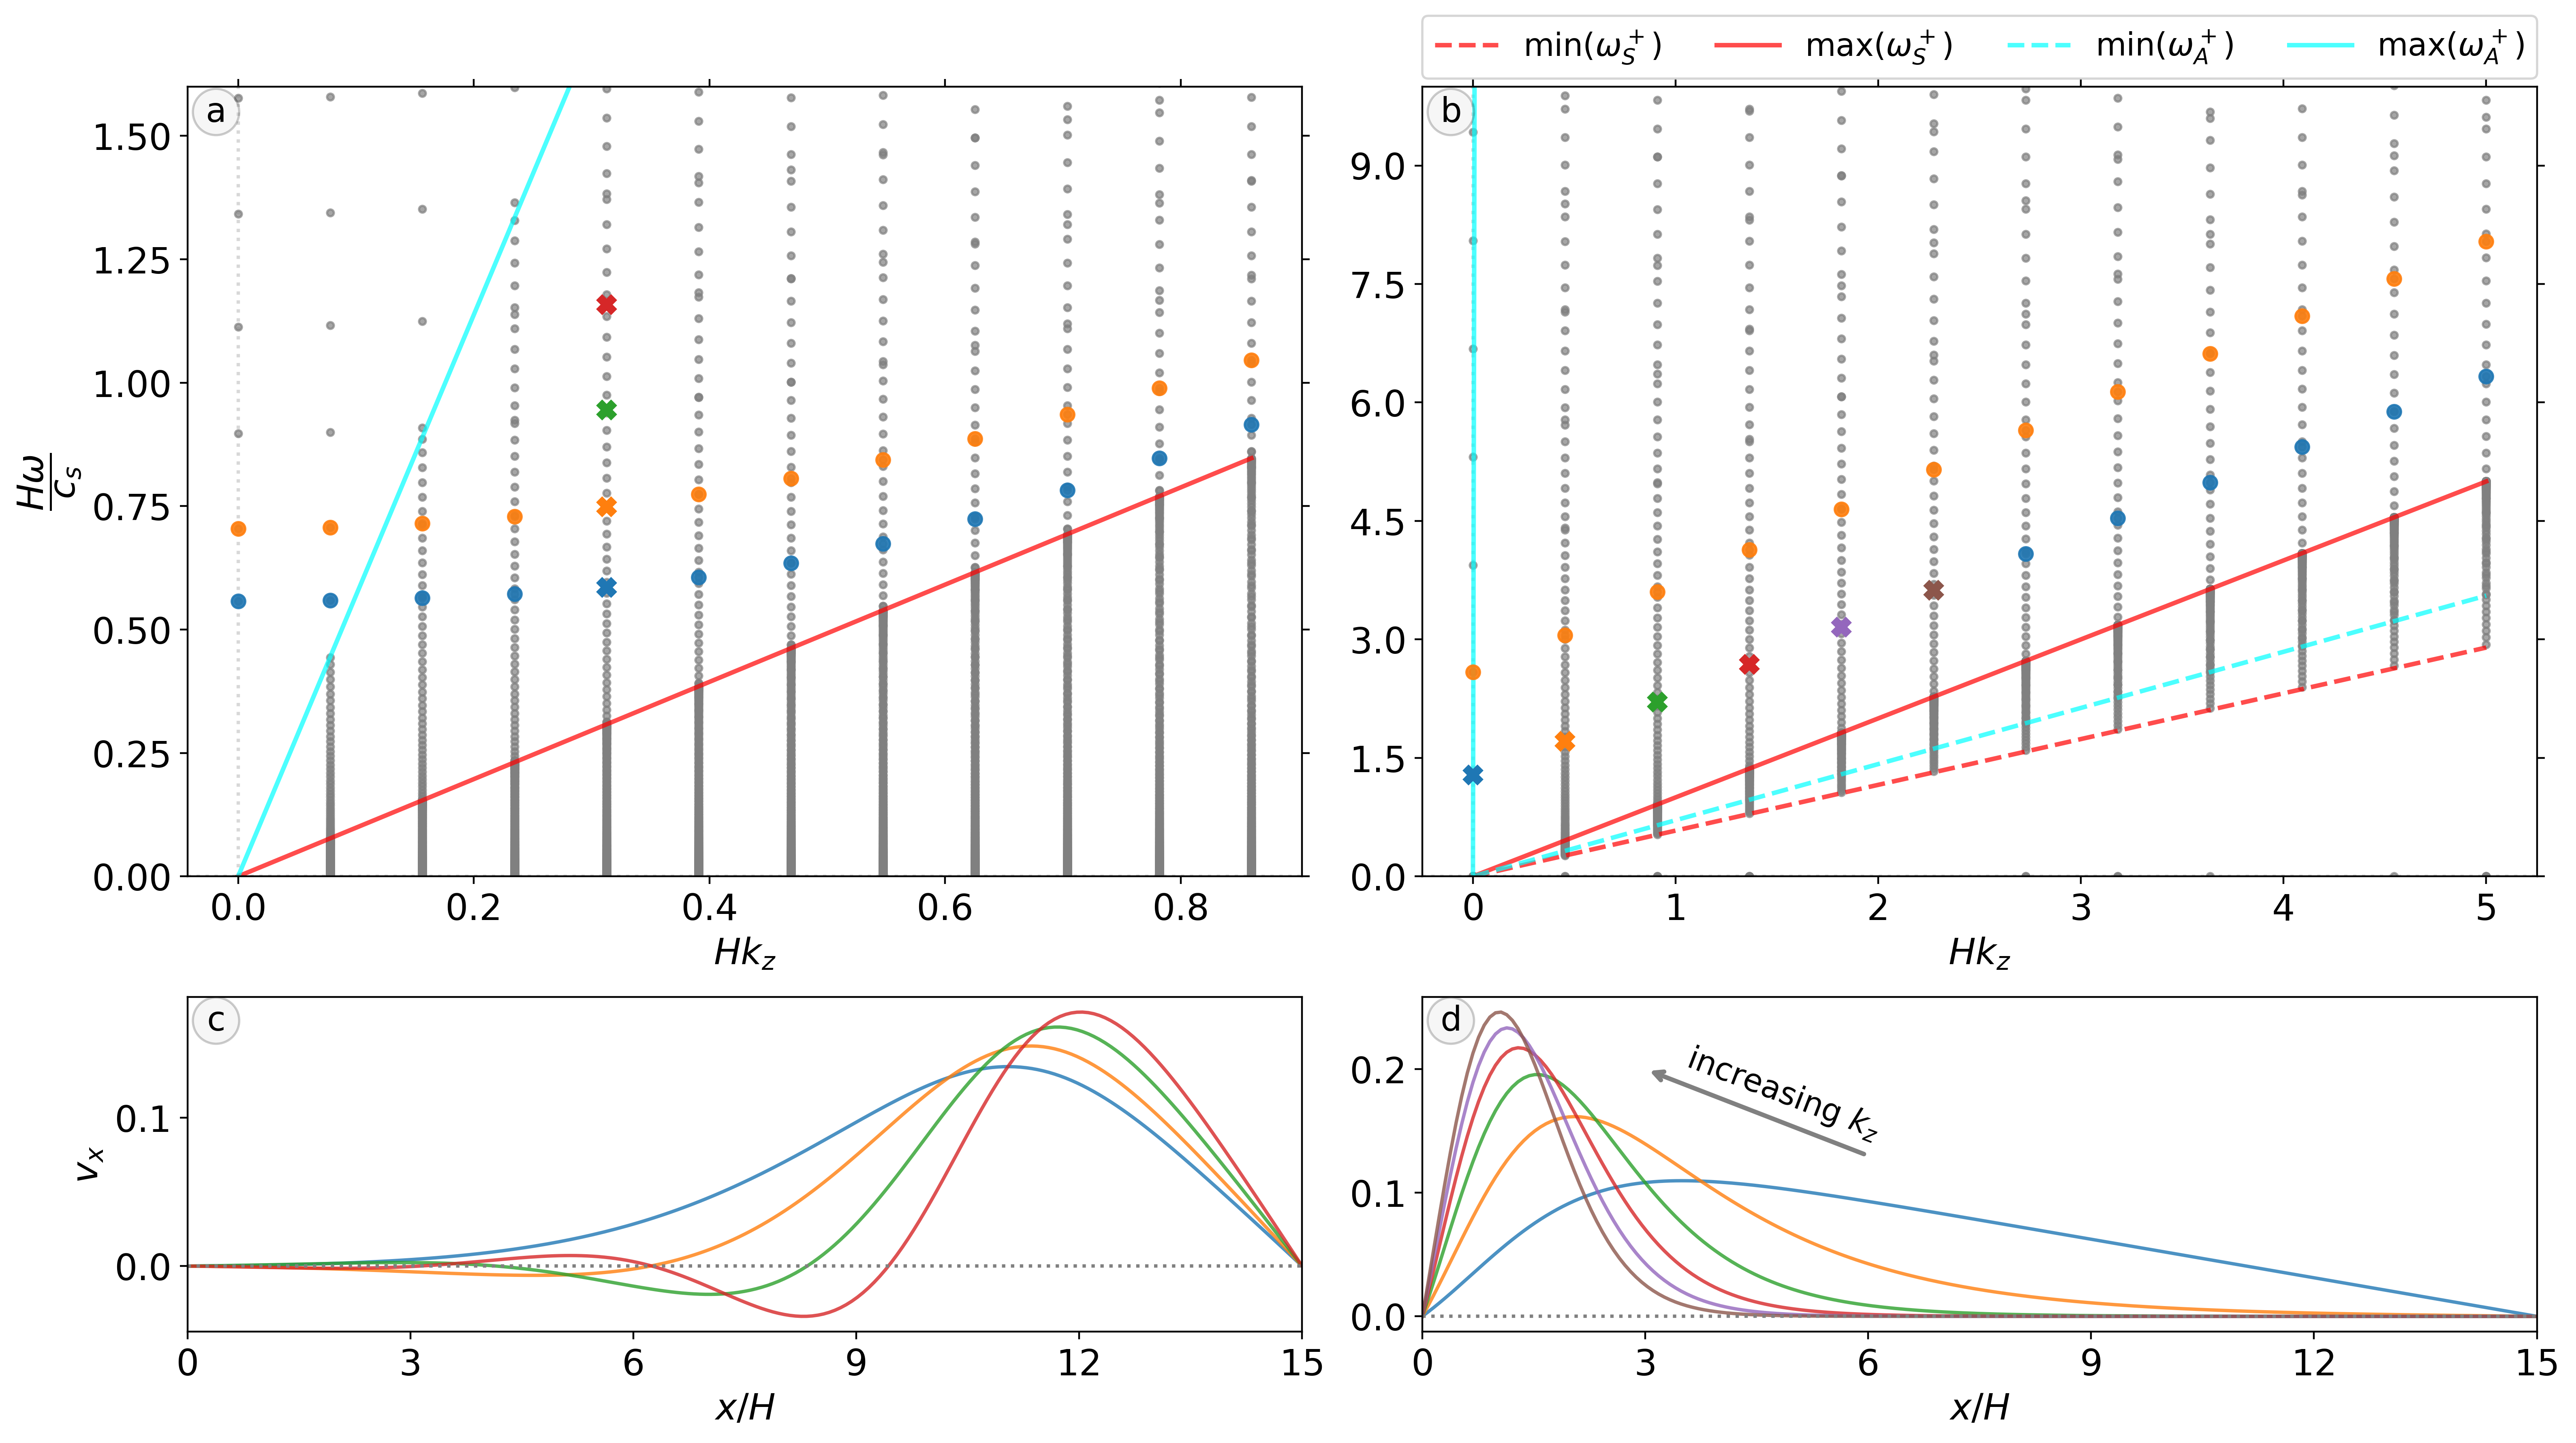
\includegraphics[width=\textwidth]{nye_thomas_ky0.png}
  \caption{
    Spectrum plots with eigenfunctions for the equilibrium in Equation \eqref{eq: nye-thomas}, for $\beta^2 = 10^{-4}$ (Panel \textbf{a}) and $\beta^2 = 0.5$ (Panel \textbf{b}), $k_y = 0$ in both cases. The blue and orange dots denote the first and second modes of the fast sequence, respectively. Panel \textbf{c}: $v_x$ eigenfunctions of the four modes annotated with a cross on Panel \textbf{a}, near $Hk_z \approx 0.3$, representing the first four modes of the fast sequence. Panel \textbf{d}: $v_x$ eigenfunctions of the modes marked with crosses on Panel \textbf{b}.
    All eigenfunctions are normalised; the colours are consistent between the panels.
  }
  \label{fig: nye-thomas-ky0}
\end{figure}

Figure \ref{fig: nye-thomas-ky0} shows spectrum plots for $\beta^2 = 10^{-4}$ (Panel a) and $\beta^2 = 0.5$ (Panel b), using the equilibrium given in Equation \eqref{eq: nye-thomas}. The full spectrum is shown with dots, where every vertical line of dots represents one {\legolas} run for that particular $k_z$ value. The first two modes of the fast sequence are annotated in blue and orange, respectively. The solid red and cyan lines denote the maxima of the slow and Alfv\'en continua, respectively, with their minima near zero (but finite). Hence, everything to the left of the cyan line in Panel a consists of purely fast modes, the region between the cyan and red line contains fast modes overlapping with the Alfv\'en continuum, and the dense collection of points below the red line corresponds to an overlapping between the slow and Alfv\'en continua. Panel c shows the $v_x$ eigenfunctions of the first four modes in the fast sequence at $H k_z \approx 0.3$ -- that is, the crossed in blue, orange, green and red, respectively, at that particular wave number. Since the magnetic field scales with the parameter $\beta$ -- where we again note that this is \emph{not} the plasma beta parameter, see Equation \eqref{eq: nye-thomas} -- this case is approximately hydrodynamic.

Panel b in Figure \ref{fig: nye-thomas-ky0} has a dynamically important magnetic field $\beta^2 = 0.5$ and shows a similar setup to Panel a. The slow and Alfv\'en continua have their minima annotated with red and cyan dashed lines, respectively. The slow continuum is constrained to a narrow band, with the Alfv\'en continuum partially overlapping. The maximum value of the latter lies far beyond the upper limit of that panel. Hence, only the modes at $k_z = 0$ represent purely fast modes; all others above the solid red line are overlapping with the Alfv\'en continuum. The first two modes of each fast sequence are again annotated in blue and orange, respectively. The $v_x$ eigenfunctions in Panel d correspond to the six annotated modes on Panel b, and they become more and more localised when $k_z$ increases.

It should be noted that the first sequence of modes in Figure \ref{fig: nye-thomas-ky0} does in fact correspond to the $k_y = 0$ and $k_z = 0$ case. This implies that the slow and Alfv\'en continua collapse to $w = 0$, and one could mistakenly be under the impression that there would be no modes present for this case. However, the Fourier dependence assumed by {\legolas}, as in Equation \eqref{eq: fourier_analysis}, does in fact allow for nontrivial $\omega$ solutions if $k_y = k_z = 0$ and $\hat{f}_1 \neq 0$, representing fast modes propagating in the $x$-direction perpendicular to the magnetic field.
Both spectra show an excellent correspondence to the plots given by \citet{nye1976}, which were obtained by analytically solving the dispersion relation. However, \citet{nye1976} never mentioned the presence of the slow and Alfv\'en continua, which were not described by their dispersion relation.


\subsection{Effects of non-parallel propagation} \label{ss: non_parallel_propagation}
As seen in Figure \ref{fig: nye-thomas-ky0}, there is an overlap between the fast mode sequence and the Alfv\'en continuum. However, when the wave vector is taken to be parallel to the magnetic field, the Alfv\'en continuum is no longer relevant in the sense that it completely decouples from the fast modes. This is the reason why that particular case becomes analytically tractable, even though the background equilibrium is homogeneous. However, there is no need to force that condition when using {\legolas}, and hence we can introduce a nonzero value for $k_y$. Even a small value of $k_y$ will have considerable effects due to the overlap with the Alfv\'en continuum, since the latter will no longer decouple, resulting in a resonance between the fast modes and the continuum.
It can be shown using a Frobenius expansion -- for a thorough discussion on this topic we refer to \citet{book_MHD} -- that this will introduce a singularity with a $\left(x - x_\text{A}\right)^{-1}$ behaviour in the eigenfunctions perpendicular to the magnetic field, where $x_\text{A}$ is the resonance radius.


\begin{figure}[t]
  \centering
  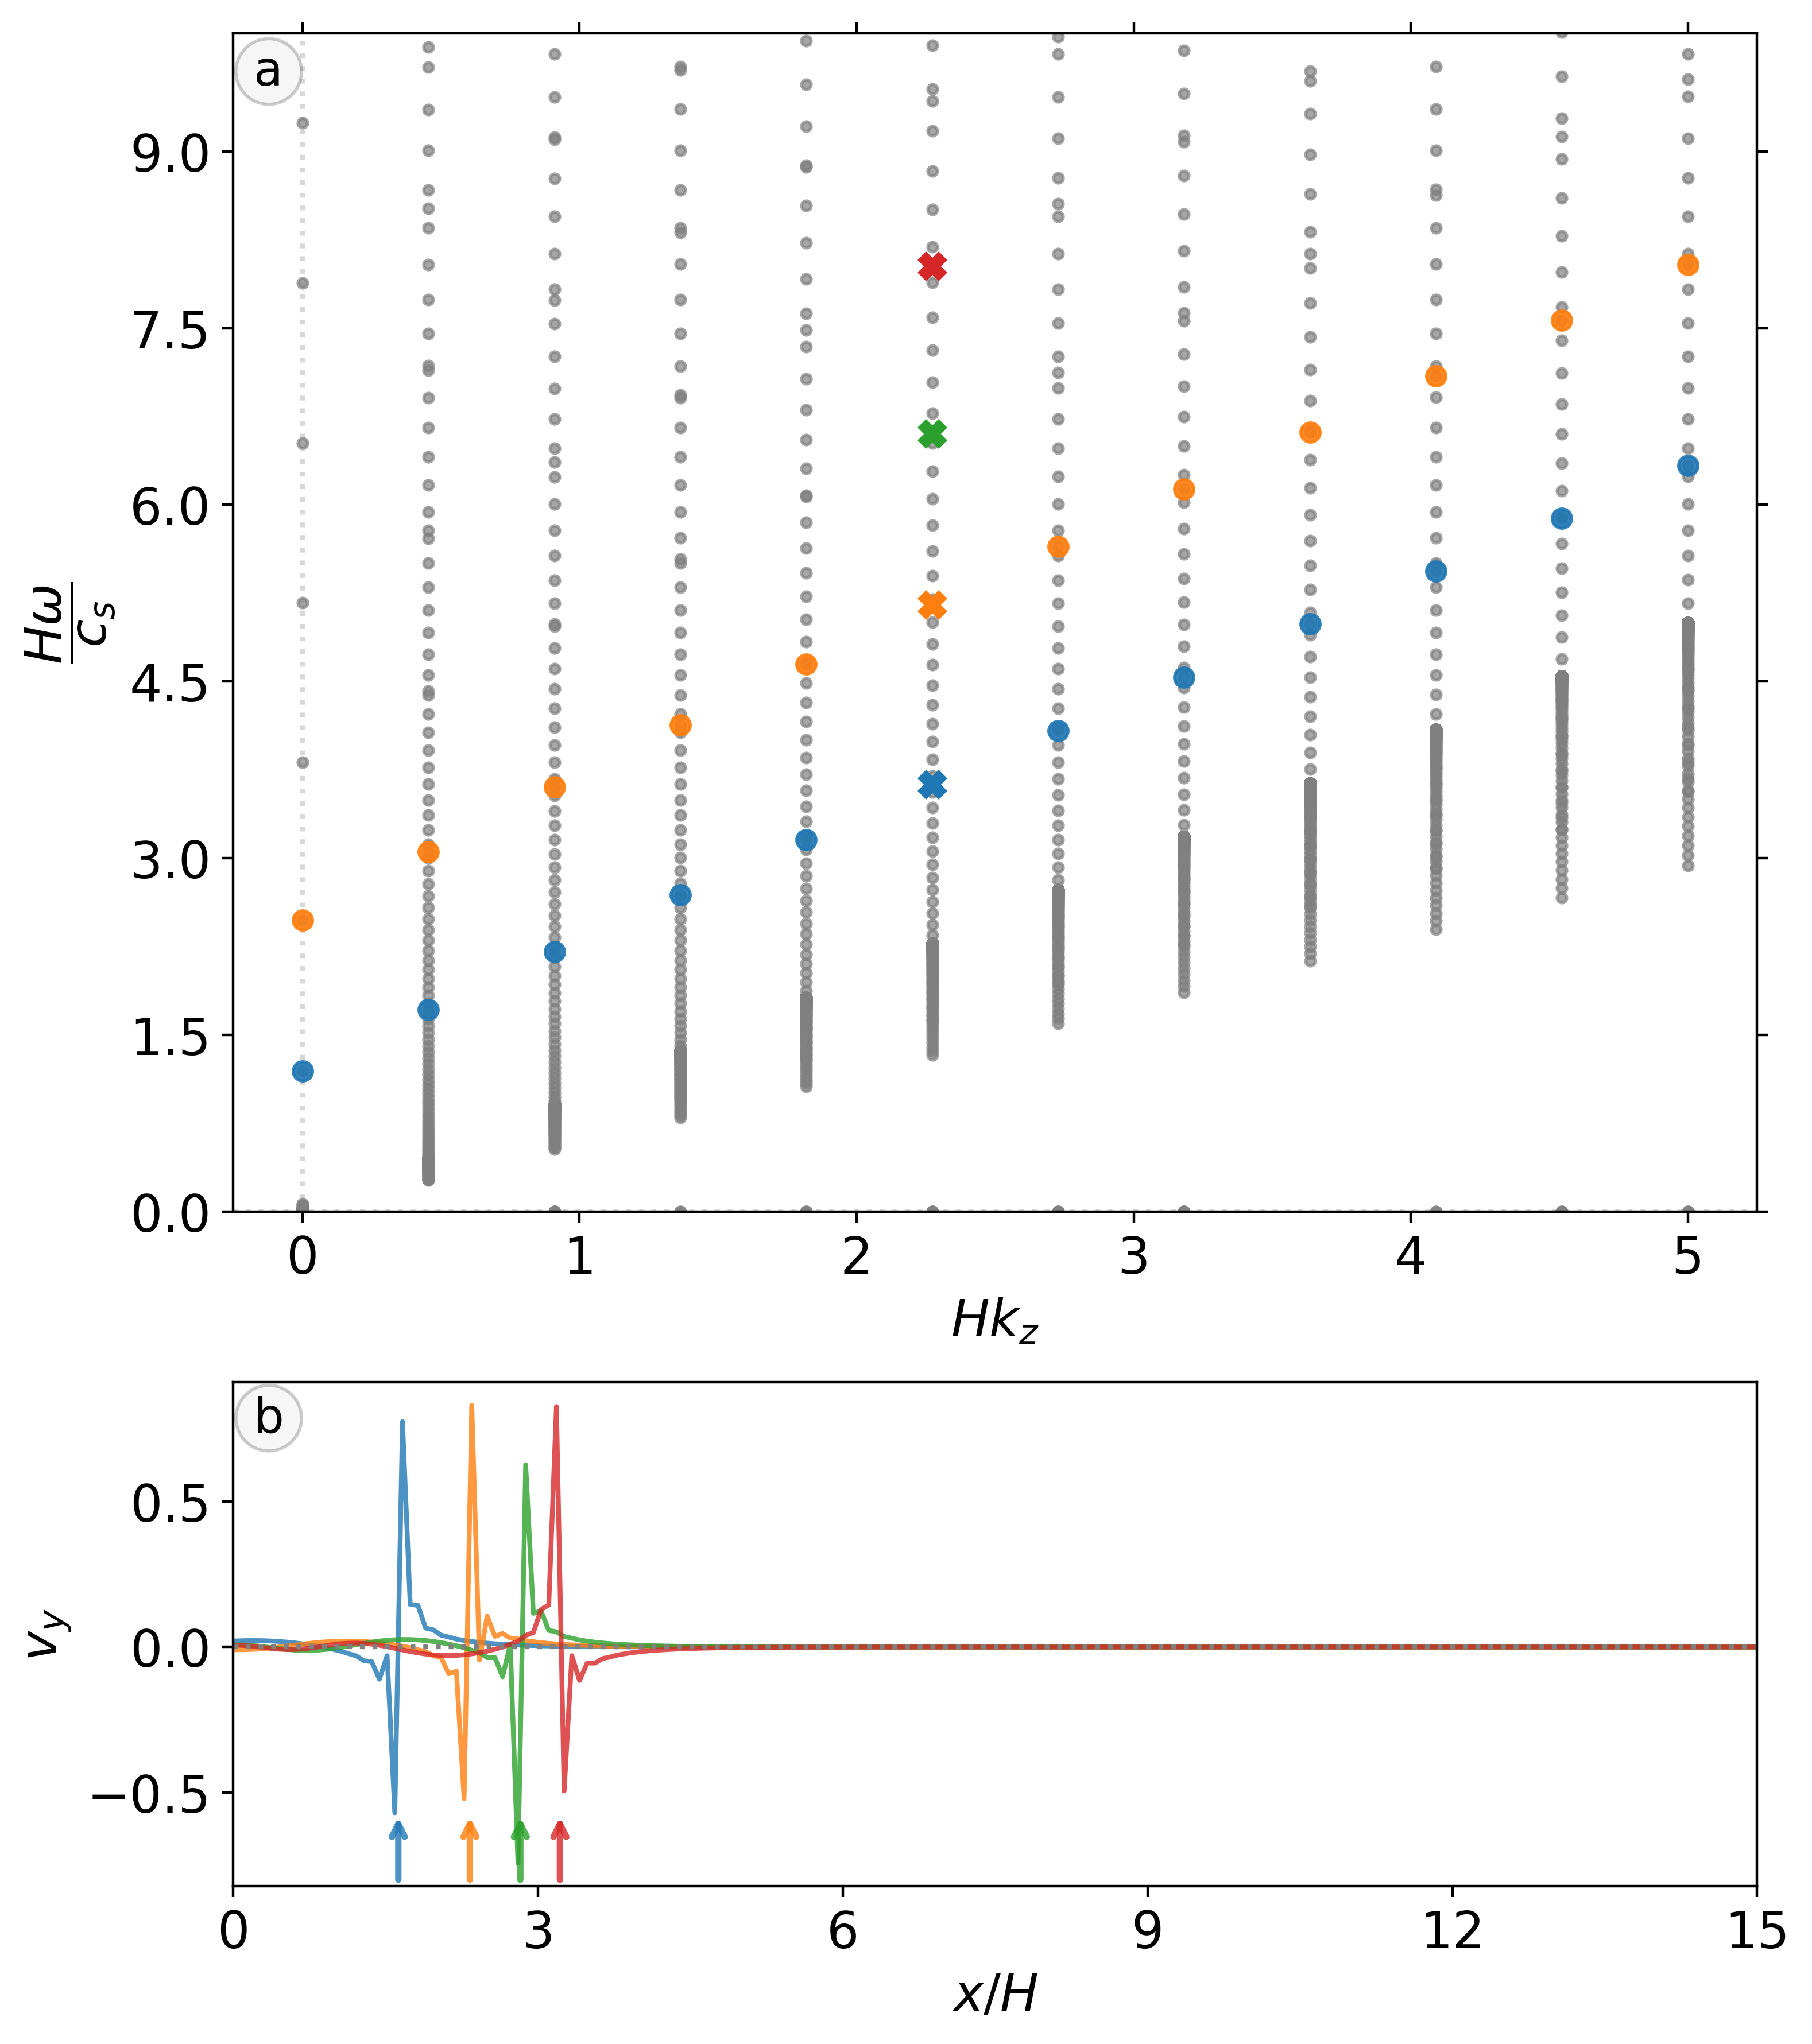
\includegraphics[width=0.65\textwidth]{nye_thomas_kynonzero.png}
  \caption{
    Panel \textbf{a}: spectrum plot for the equilibrium in Equation \eqref{eq: nye-thomas} with $\beta^2 = 0.5$ and
    $k_y = 0.05$. Blue and orange dots denote the first and second mode of the fast sequences, respectively.
    Panel \textbf{b} shows $v_y$ eigenfunctions of the four modes annotated with crosses in the fast sequence at
    $H k_z \approx 2.2$, clearly showing the $1/x$ behaviour at $x = x_\text{A}$ due to overlap and resonance with the Alfv\'en continuum. The arrows denotes the resonance radius predicted by Equation \eqref{eq: resonance_radius}.
  }
  \label{fig: nye-thomas-kynonzero}
\end{figure}

In the case considered here it is actually possible to make an estimate of this radius, by starting from the regular expression for the Alfv\'en continuum $\omega_\text{A}^+ = \left(\bk \cdot \bb_0\right)/ \sqrt{\rho(x)}$. Since the magnetic field is homogeneous, this expression can be inverted to yield $x_\text{A}$ as a function of frequency:
\begin{equation} \label{eq: resonance_radius}
  x_\text{A} = 2 H \ln\left(\frac{\omega}{k_z B_{0z}}\right),
\end{equation}
where we used the fact that $\rho_{00} = 1$ and the magnetic field is aligned with the $z$-axis. If we now substitute the frequency of the fast mode under consideration, Equation \eqref{eq: resonance_radius} will give an indication where in the eigenfunction the $1/x$ singularity will occur. Naturally, this also implies that the location of this singularity is frequency and wavenumber dependent, resulting in a larger $x_\text{A}$ when the frequency increases; that is, for higher modes in the sequence, and a smaller $x_\text{A}$ when $k_z$ increases.

Figure \ref{fig: nye-thomas-kynonzero} shows the same setup as Panel b in Figure \ref{fig: nye-thomas-ky0}, but now with $k_y = 0.05$. As seen on Panel a the spectrum itself is practically unaffected, the first two modes of each fast sequence are again annotated. Panel b shows the $v_y$ eigenfunctions for the four modes at $H k_z \approx 2.2$, clearly showing the $1/x$ singular behaviour. The arrows denote the estimated value for the resonance radius $x_\text{A}$ according to Equation \eqref{eq: resonance_radius} in the same colour as its eigenfunction, with values given by $x_\text{A} \approx 1.63$, $x_\text{A} \approx 2.33$, $x_\text{A} \approx 2.83$ and $x_\text{A} \approx 3.22$ for the first, second, third and fourth mode of the fast sequence at that value for $k_z$, respectively. Since these modes correspond fo the same fast mode sequence, and thus have the same value for $k_z$, we indeed see the singularity moving to the right on the figure, locating itself at larger $x_\text{A}$ values for higher mode numbers.

It should be noted that these eigenfunctions do not show a ``real'' $1/x$ behaviour in the sense that the eigenfunctions rather show a spiked oscillation instead of extending towards infinity. This is due to {\legolas} trying to approximate those eigenfunctions with the limited number of gridpoints at its disposal. The more the resolution is increased, the more this singular $1/x$ profile will be resolved. This truly singular behaviour due to this resonance is particular to ideal MHD, but we could also activate resistive terms in {\legolas}, to then get a fully resolved complex eigenfrequency at finite resistivity with a spatially resolved eigenfunction behaviour.


\subsection{Inclusion of non-adiabatic effects} \label{ss: non_adiabatic_effects}
As a final extension to this rather simple model, we again consider the $\beta^2 = 0.5$ configuration from Section \ref{ss: parallel_propagation} but now include non-adiabatic effects: thermal conduction parallel to the magnetic field lines and optically thin radiative losses based on the {\spexdm} cooling curve given in Figure \ref{fig: coolingcurves}. Since this will cause the introduction of complex eigenfrequencies, we now focus on the full spectrum for $k_z = 2$ and $k_y = 0$. Figure \ref{fig: nye-thomas-nonadiabatic} shows the corresponding spectrum for 250 gridpoints in Panel a, whereas Panel b shows the exact same spectrum but without non-adiabatic effects for comparison. The thermal, slow, and Alfv\'en continua are annotated in green, red, and cyan, respectively. By comparing Panels a and b it can be seen that the thermal continuum shifts from its marginal solution in the adiabatic case to the dense band of modes on the imaginary axis as given by Equation \eqref{eq: slow_thermal_continuum}, in this case with both a stable and unstable part. The same holds true for the slow continuum, which shifts from its purely real adiabatic solution to an intricate loop in the complex plane, becoming partially unstable. The inset on Panel a zooms in on the slow sequence, revealing a single discrete mode annotated by a pink cross, with the imaginary part of its $\rho$ and $v_x$ eigenfunctions shown in pink on Panels c, both showing a strong oscillation in the lower regions of the slab. This discrete eigenvalue represents a global unstable slow mode since it is not part of the continuum, although it can be linked to an internal extremum as shown in Figure \ref{fig: nye-thomas-continua}.

\begin{figure}[t]
  \centering
  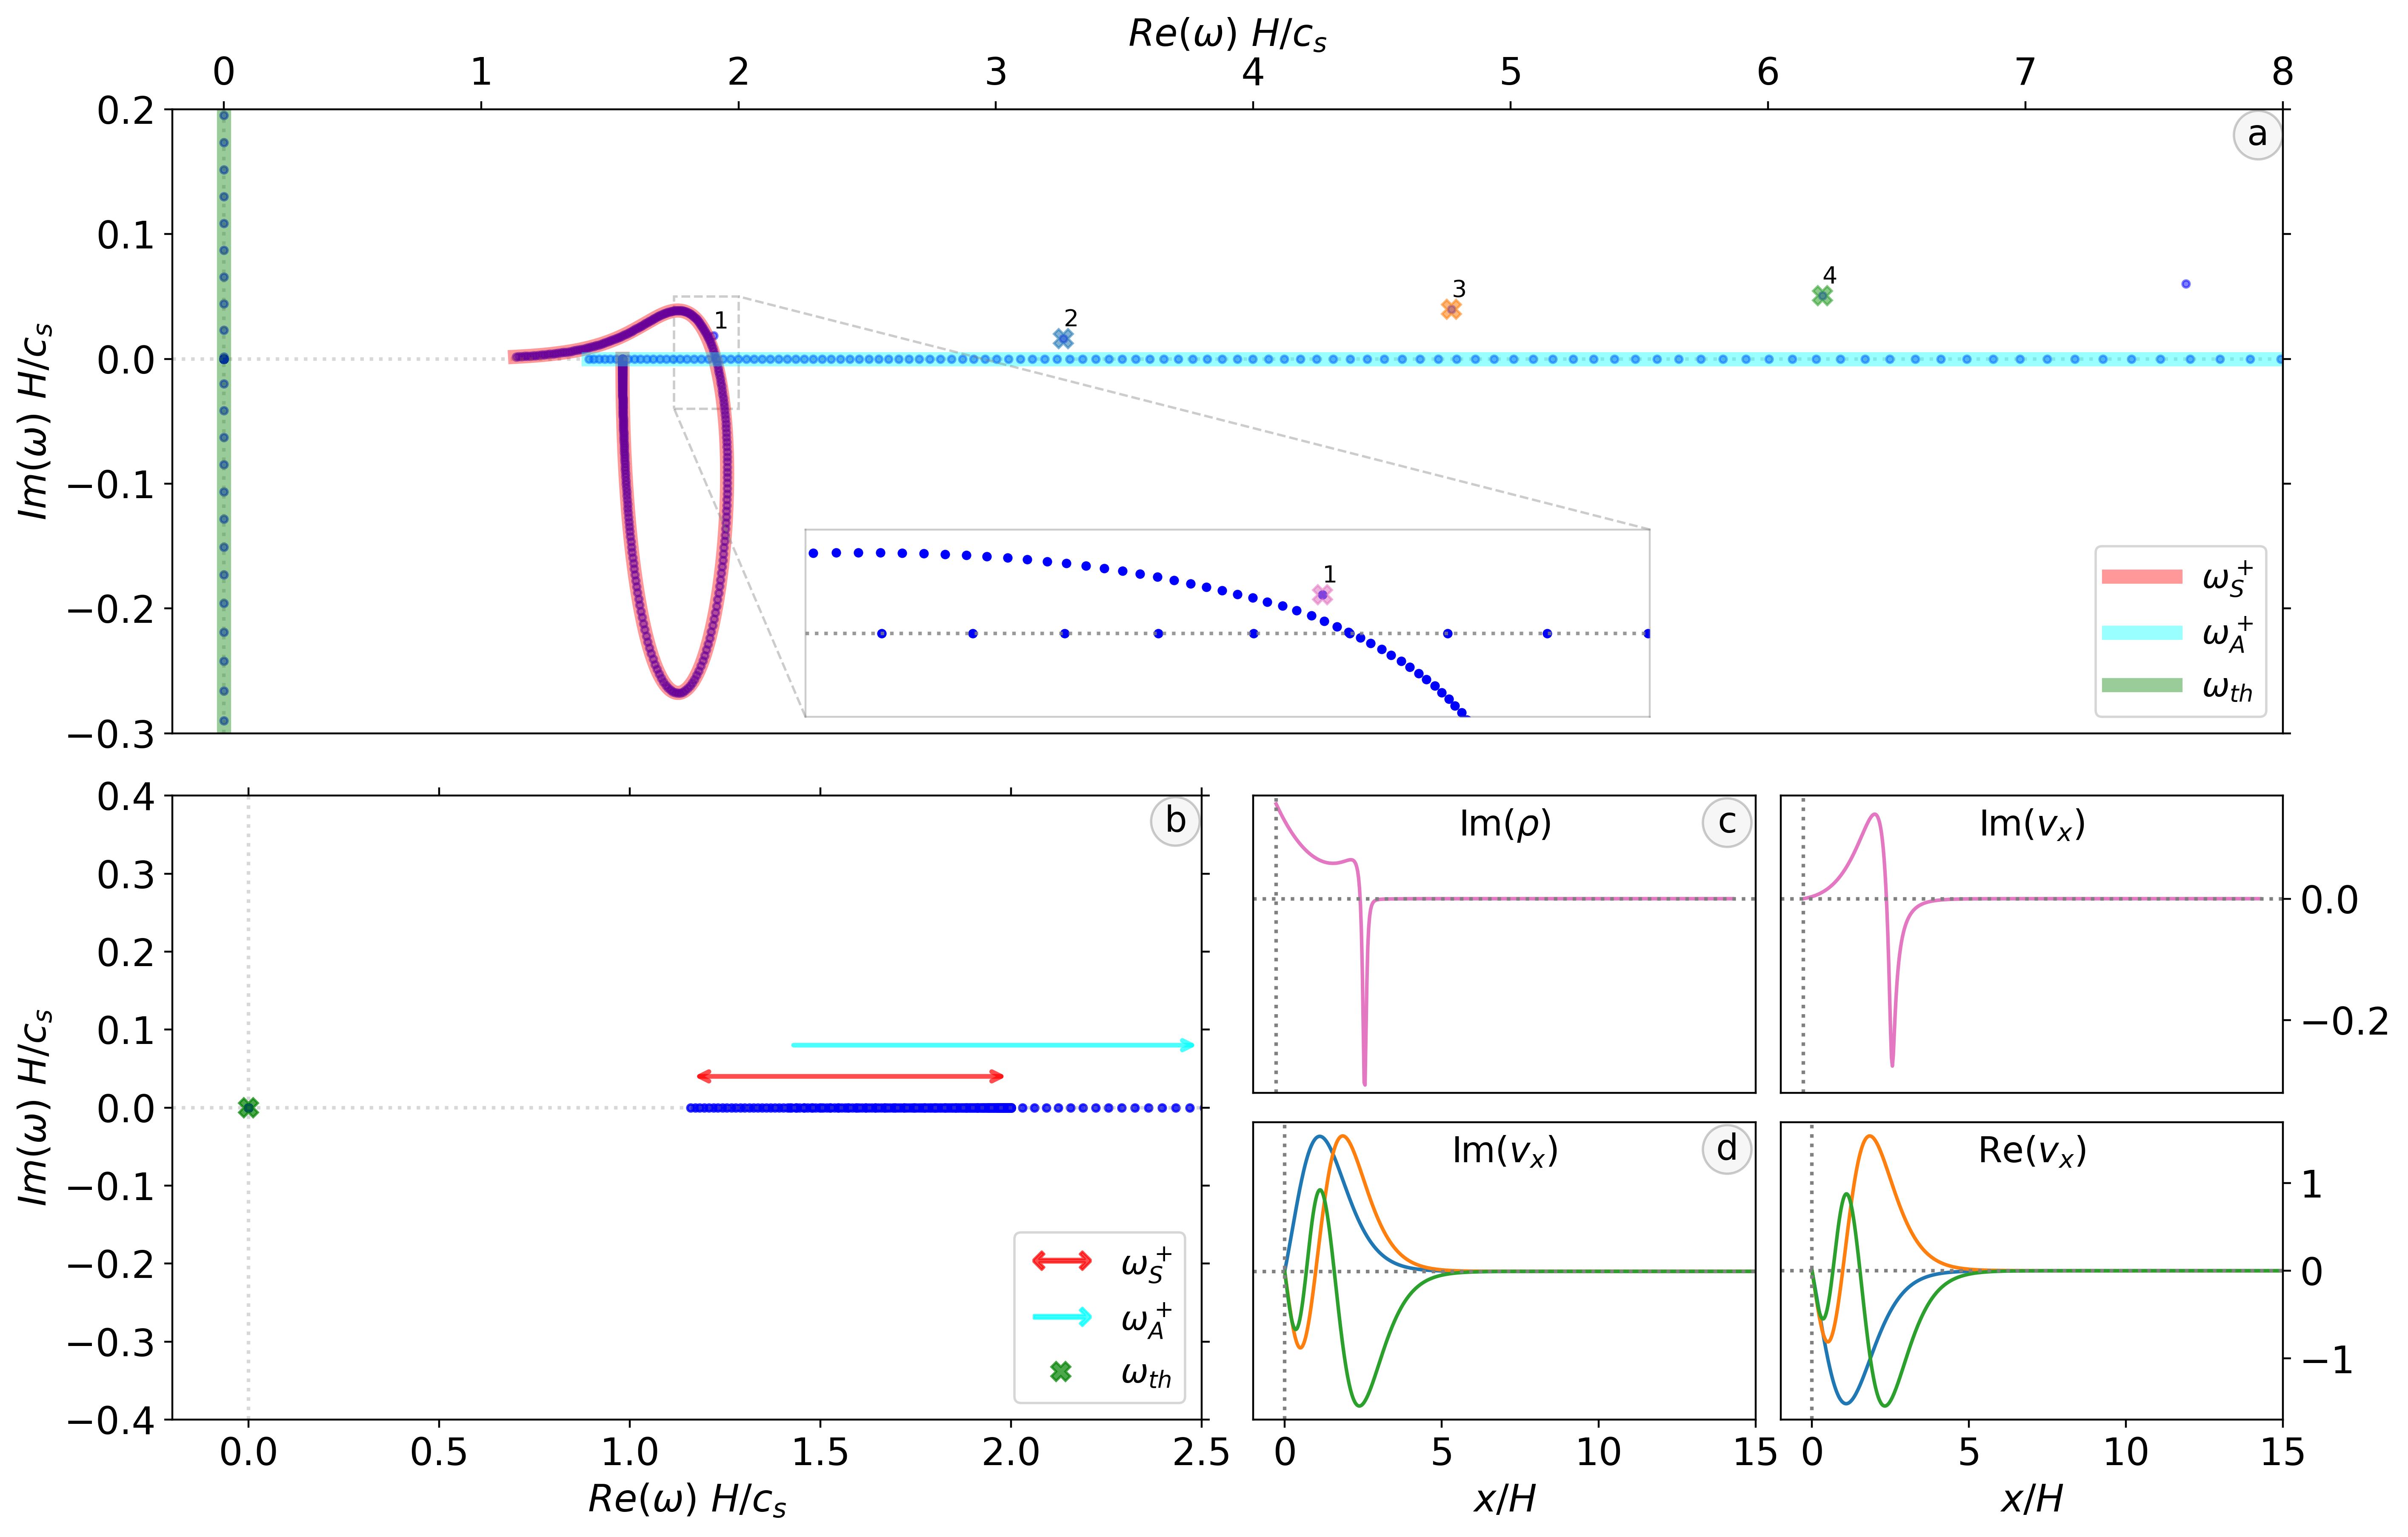
\includegraphics[width=\textwidth]{nye_thomas_nonadiabatic.png}
  \caption{
    Spectra and eigenfunctions for the $\beta^2 = 0.5$ setup in Section \ref{ss: parallel_propagation}, with non-adiabatic effects included. Panel \textbf{a}: enlargement near the slow sequence, showing (part of) the thermal, slow, and Alfv\'en continua in green, red, and cyan, respectively, along with four unstable modes from the fast sequence. Inset: further enlargement on the slow continuum, revealing a single discrete mode.
    Panel \textbf{b}: same as in Panel \textbf{a}, but without non-adiabatic effects. Panels \textbf{c}: $\rho$ (left) and $v_x$ (right) eigenfunctions of the discrete mode annotated in the inset. Panels \textbf{d}: $v_x$ eigenfunctions for the three fast modes annotated on Panel \textbf{a}. All eigenfunctions are normalised.
  }
  \label{fig: nye-thomas-nonadiabatic}
\end{figure}

The first few (unstable) modes of the fast sequence in Panel a overlap with the Alfv\'en continuum, which is decoupled due to $k_y$ being zero. The real part of these fast modes is approximately equal to the values shown on Figure \ref{fig: nye-thomas-ky0}, Panel b, where the first and second coloured modes on that panel would correspond to modes 2 and 3 on Figure \ref{fig: nye-thomas-nonadiabatic}, Panel a; the imaginary part is non nonzero due to the non-adiabatic effects included. The $v_x$ eigenfunctions of these fast modes are given in Panels d. All eigenfunctions on this figure are calculated using a shift-invert method near the eigenvalue of interest.

\begin{figure}[t]
  \centering
  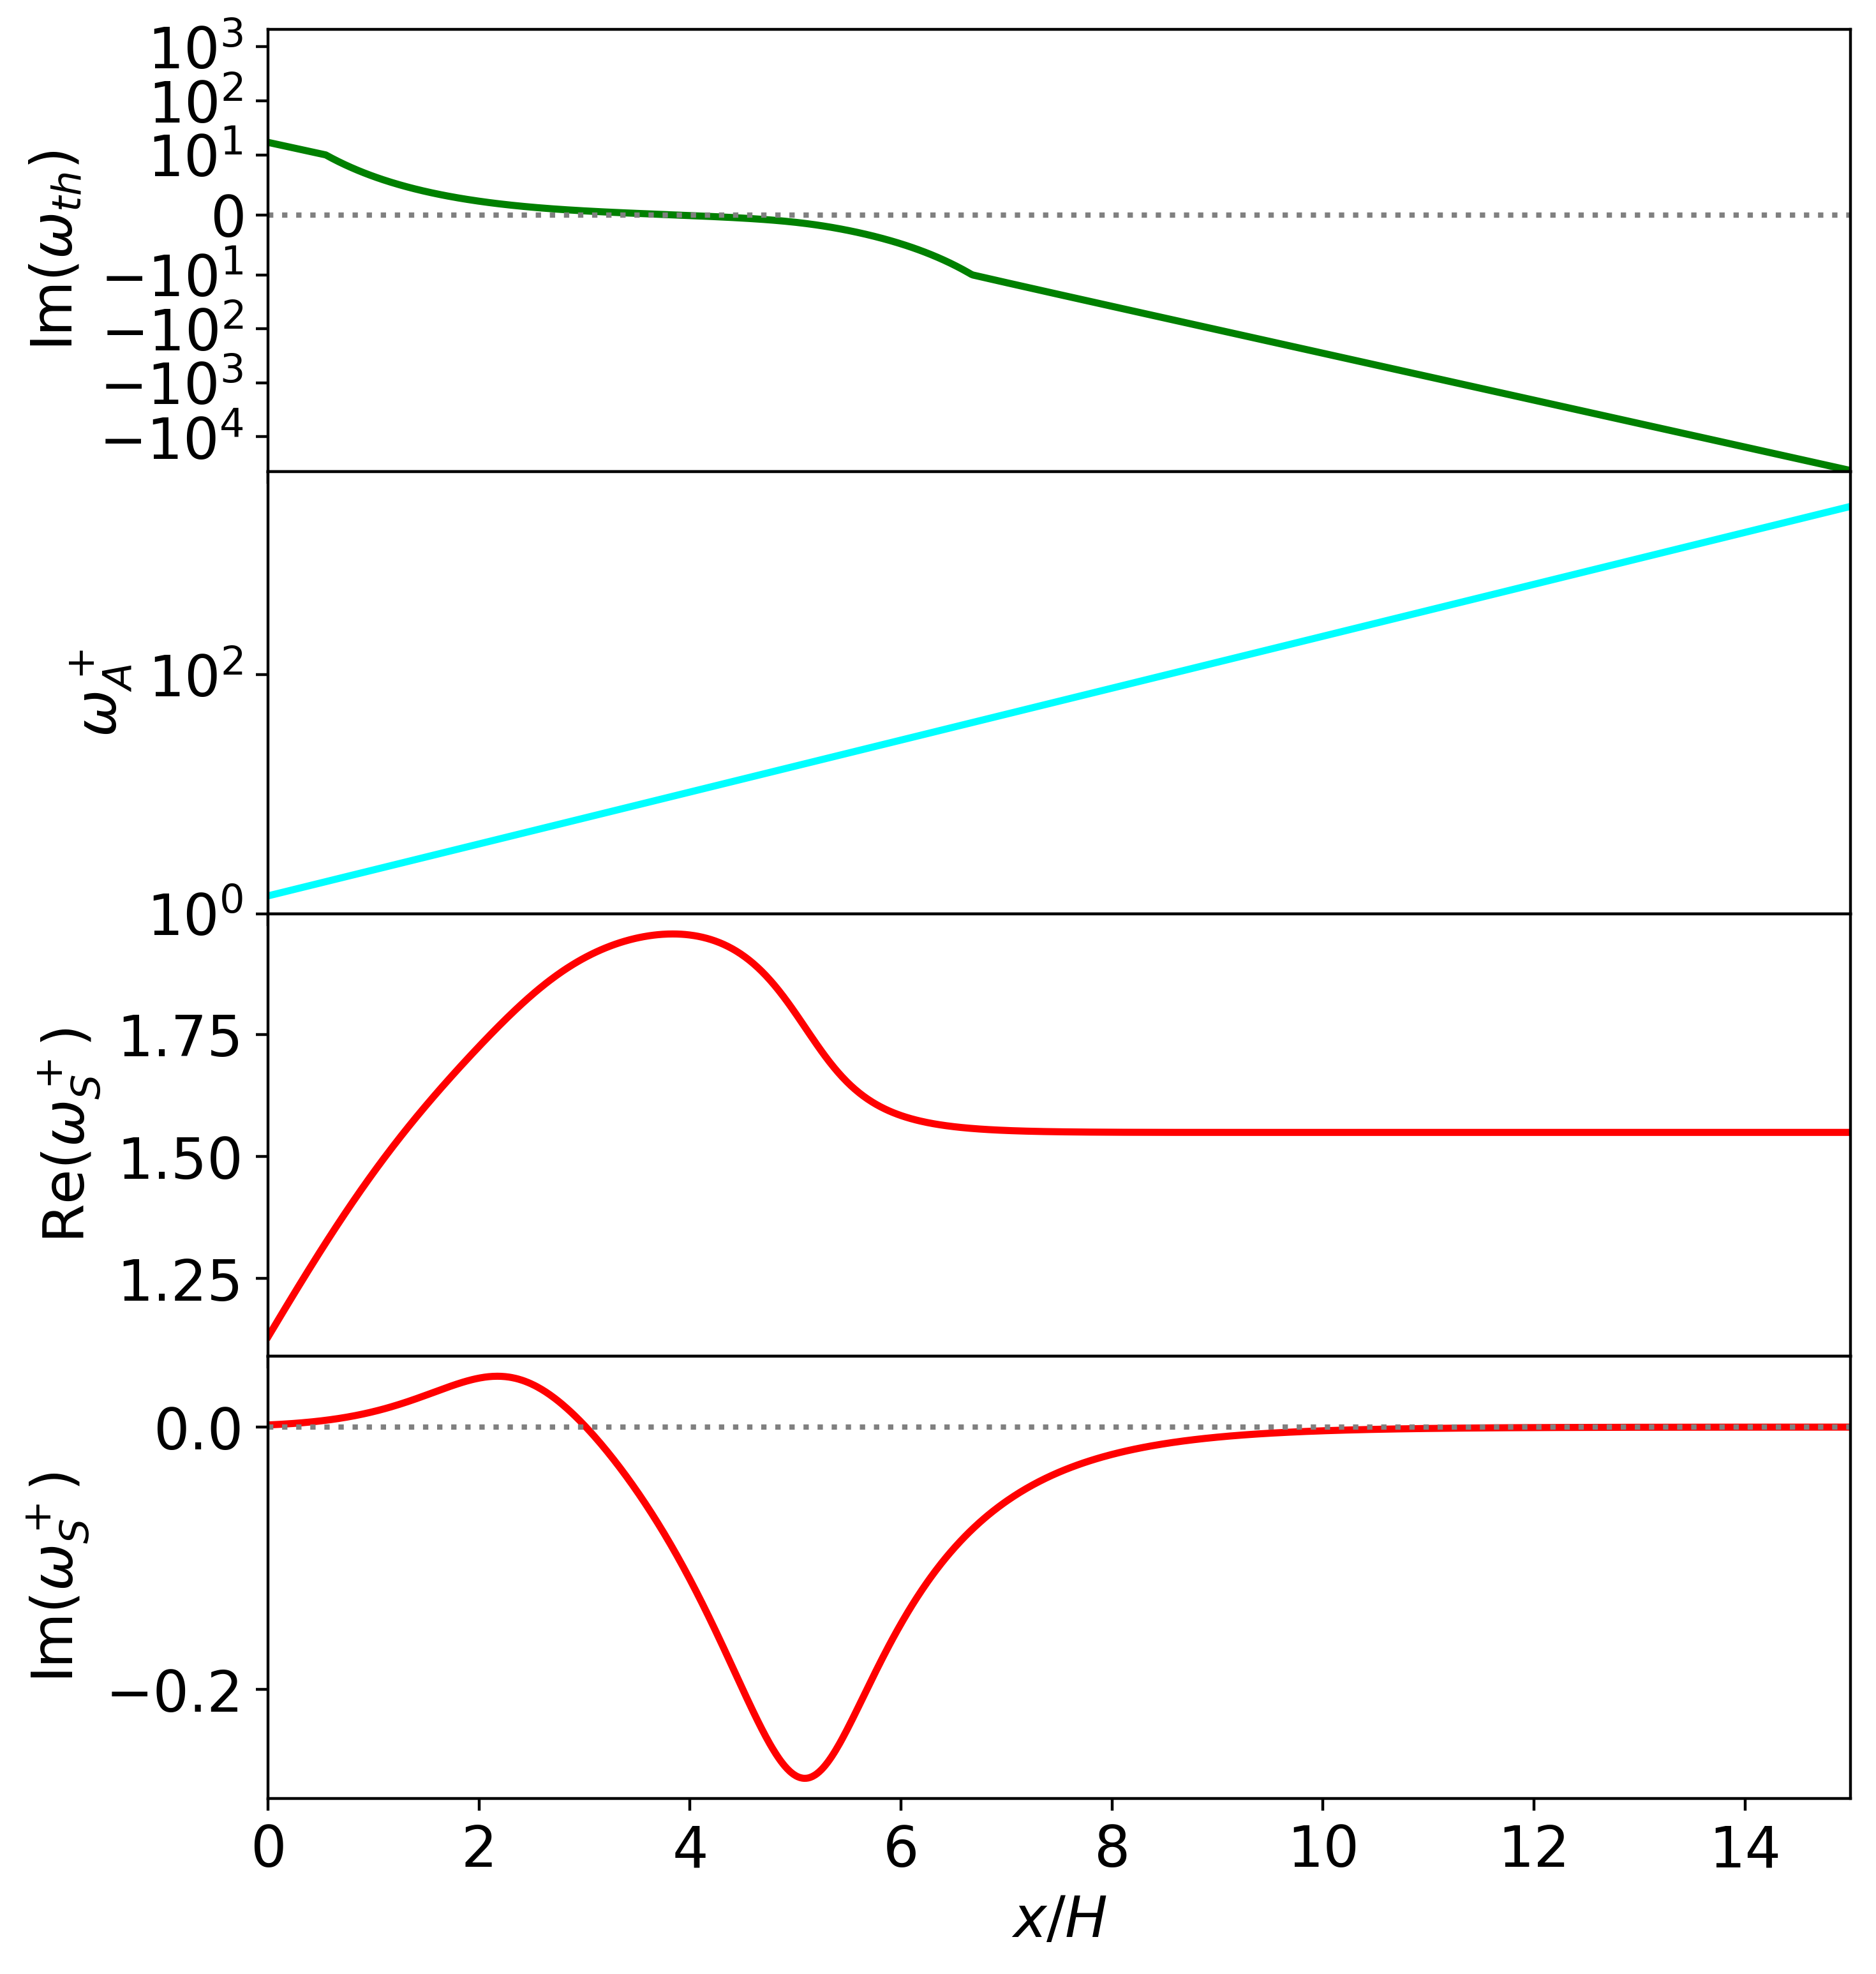
\includegraphics[width=0.65\textwidth]{nye_thomas_continua.png}
  \caption{
    The thermal (green), Alfv\'en (cyan), and slow (red) continua as a function of height, for the non-adiabatic case shown in Figure \ref{fig: nye-thomas-nonadiabatic}. The slow continuum shows an internal extremum. All continua are rescaled to $H / \soundspeed$, similar to the other figures in this Section.
  }
  \label{fig: nye-thomas-continua}
\end{figure}

Figure \ref{fig: nye-thomas-continua} shows all continua corresponding to the non-adiabatic case discussed here, rescaled using the scale height and sound speed in order to be consistent with Figure \ref{fig: nye-thomas-nonadiabatic}. The thermal continuum (green) has clear variation, but no internal extrema. The slow continuum on the other hand does have an internal maximum in its real part, which can be linked back to the unstable discrete mode we found, shown on the inset on Panel a, Figure \ref{fig: nye-thomas-nonadiabatic}. Note that this simple magnetised atmosphere model thus already gives us unstable parts in the thermal and slow continuum, and gives overstable discrete modes linked to both the slow and the fast mode sequences.

What this implies for an initial value problem where this particular atmosphere would be realised in a numerical nonlinear MHD simulation with all the non-adiabatic effects included is as follows: since the thermal continuum has an unstable part that is almost two orders of magnitude larger than the unstable parts of either the slow or fast modes, one would expect that the most unstable thermal mode(s) would dominate the thermal behaviour, since these have the largest growth rates. Physically, this would mean that any perturbation would immediately lead to an in-situ condensation. However, the possibility of some form of coalescence between the unstable slow and fast modes and the thermal modes (or even a combination of all three) can not be excluded. In that case a cool and dense condensation will still form, but the way this happens (and it subsequent dynamics) may be much more intricate than a ``simple'' in-place condensation.


\section{A realistic solar atmosphere model} \label{sec: solar_atmosphere}
We now extend the study of waves and instabilities in stratified, magnetised atmospheres to a fully realistic atmosphere description. This requires us to specify the equilibrium (Section \ref{ss: atmosphere_model}), after which we look at the non-adiabatic continua governed by Equation \eqref{eq: slow_thermal_continuum}. Then, we show full MHD spectra for the solar atmosphere, focusing on specific regions of interest. All models in this Section assume solid wall boundaries on both sides of the stratified slab.

\subsection{The stratified, magnetised atmosphere} \label{ss: atmosphere_model}
As discussed before in Section \ref{ss: equilibrium conditions} the choice of equilibrium profile together with the system of equations considered yields two conditions for the background, here the equations governing the force-balanced state are given by \eqref{eq: force_equilibrium}--\eqref{eq: thermal_equilibrium}. In the cases discussed in this Chapter we ignore flow effects, such that the equations simplify considerably:
\begin{gather}
  \left(\rho_0 T_0 + \frac{1}{2}B_0^2\right)' = -\rho_0 g, \label{eq: simple_force_balance} \\
  \left(\kappaperp T_0'\right)' = \rho_0 \HLF_0, \label{eq: simple_thermal_balance}
\end{gather}
where as before the prime denotes the derivative, in this case with respect to the height coordinate $x$ since we are looking at Cartesian geometries (and thus $\eps = 1$ and $\eps' = 0$). The heating function $\HLFheat$ is assumed to be constant such that it balances out radiative losses, perpendicular thermal conduction is ignored, hence Equation \eqref{eq: simple_thermal_balance} is naturally satisfied and thermal balance is ensured.

In the model considered here, we assume a Cartesian slab parallel to the solar surface infinitely extended along the $y$- and $z$-directions, with a variation along $x$ in the equilibrium quantities and an external gravitational field directed downward towards the solar surface. For the temperature profile we use a solar atmospheric model proposed by \citet{avrett2008}, which is based on detailed radiative transfer calculations and observations. This profile is interpolated at high resolution using a local second-order polynomial approximation, similar to how the radiative cooling curves are treated (see Figure \ref{fig: coolingcurves}). For the gravitational field we assume the following profile,
\begin{equation} \label{eq: solar_gravity}
  g(x) = \gdot \left(\frac{\Rdot}{\Rdot + x}\right)^2,
\end{equation}
where $\gdot = 274$ ms$^{-2}$ denotes the solar gravitational constant and $\Rdot = 6.96 \times 10^{10}$ cm the solar radius. The magnetic field is assumed to be uniform and horizontal (aligned along $z$). Note that this is similar to the analytic case discussed before, and it still avoids horizontal magnetic fields that shear or vary in magnitude with height. Also, no vertical magnetic field components are considered here ($B_{01} = 0$). Since this kind of equilibrium is numerical and relies on interpolated temperature profiles, the density profile has to be calculated in order to achieve a force-balanced state. Once the temperature, gravity, and magnetic field profiles are chosen, Equation \eqref{eq: simple_force_balance} can be rewritten in terms of density as the following first order differential equation
\begin{equation} \label{eq: density_ode}
  \rho_0'(x) = -\frac{T_0'(x) + g(x)}{T_0(x)}\rho_0(x) - \frac{B_{0y}(x)B_{0y}'(x) + B_{0z}(x)B_{0z}'(x)}{T_0(x)}.
\end{equation}
\begin{figure}[t]
  \centering
  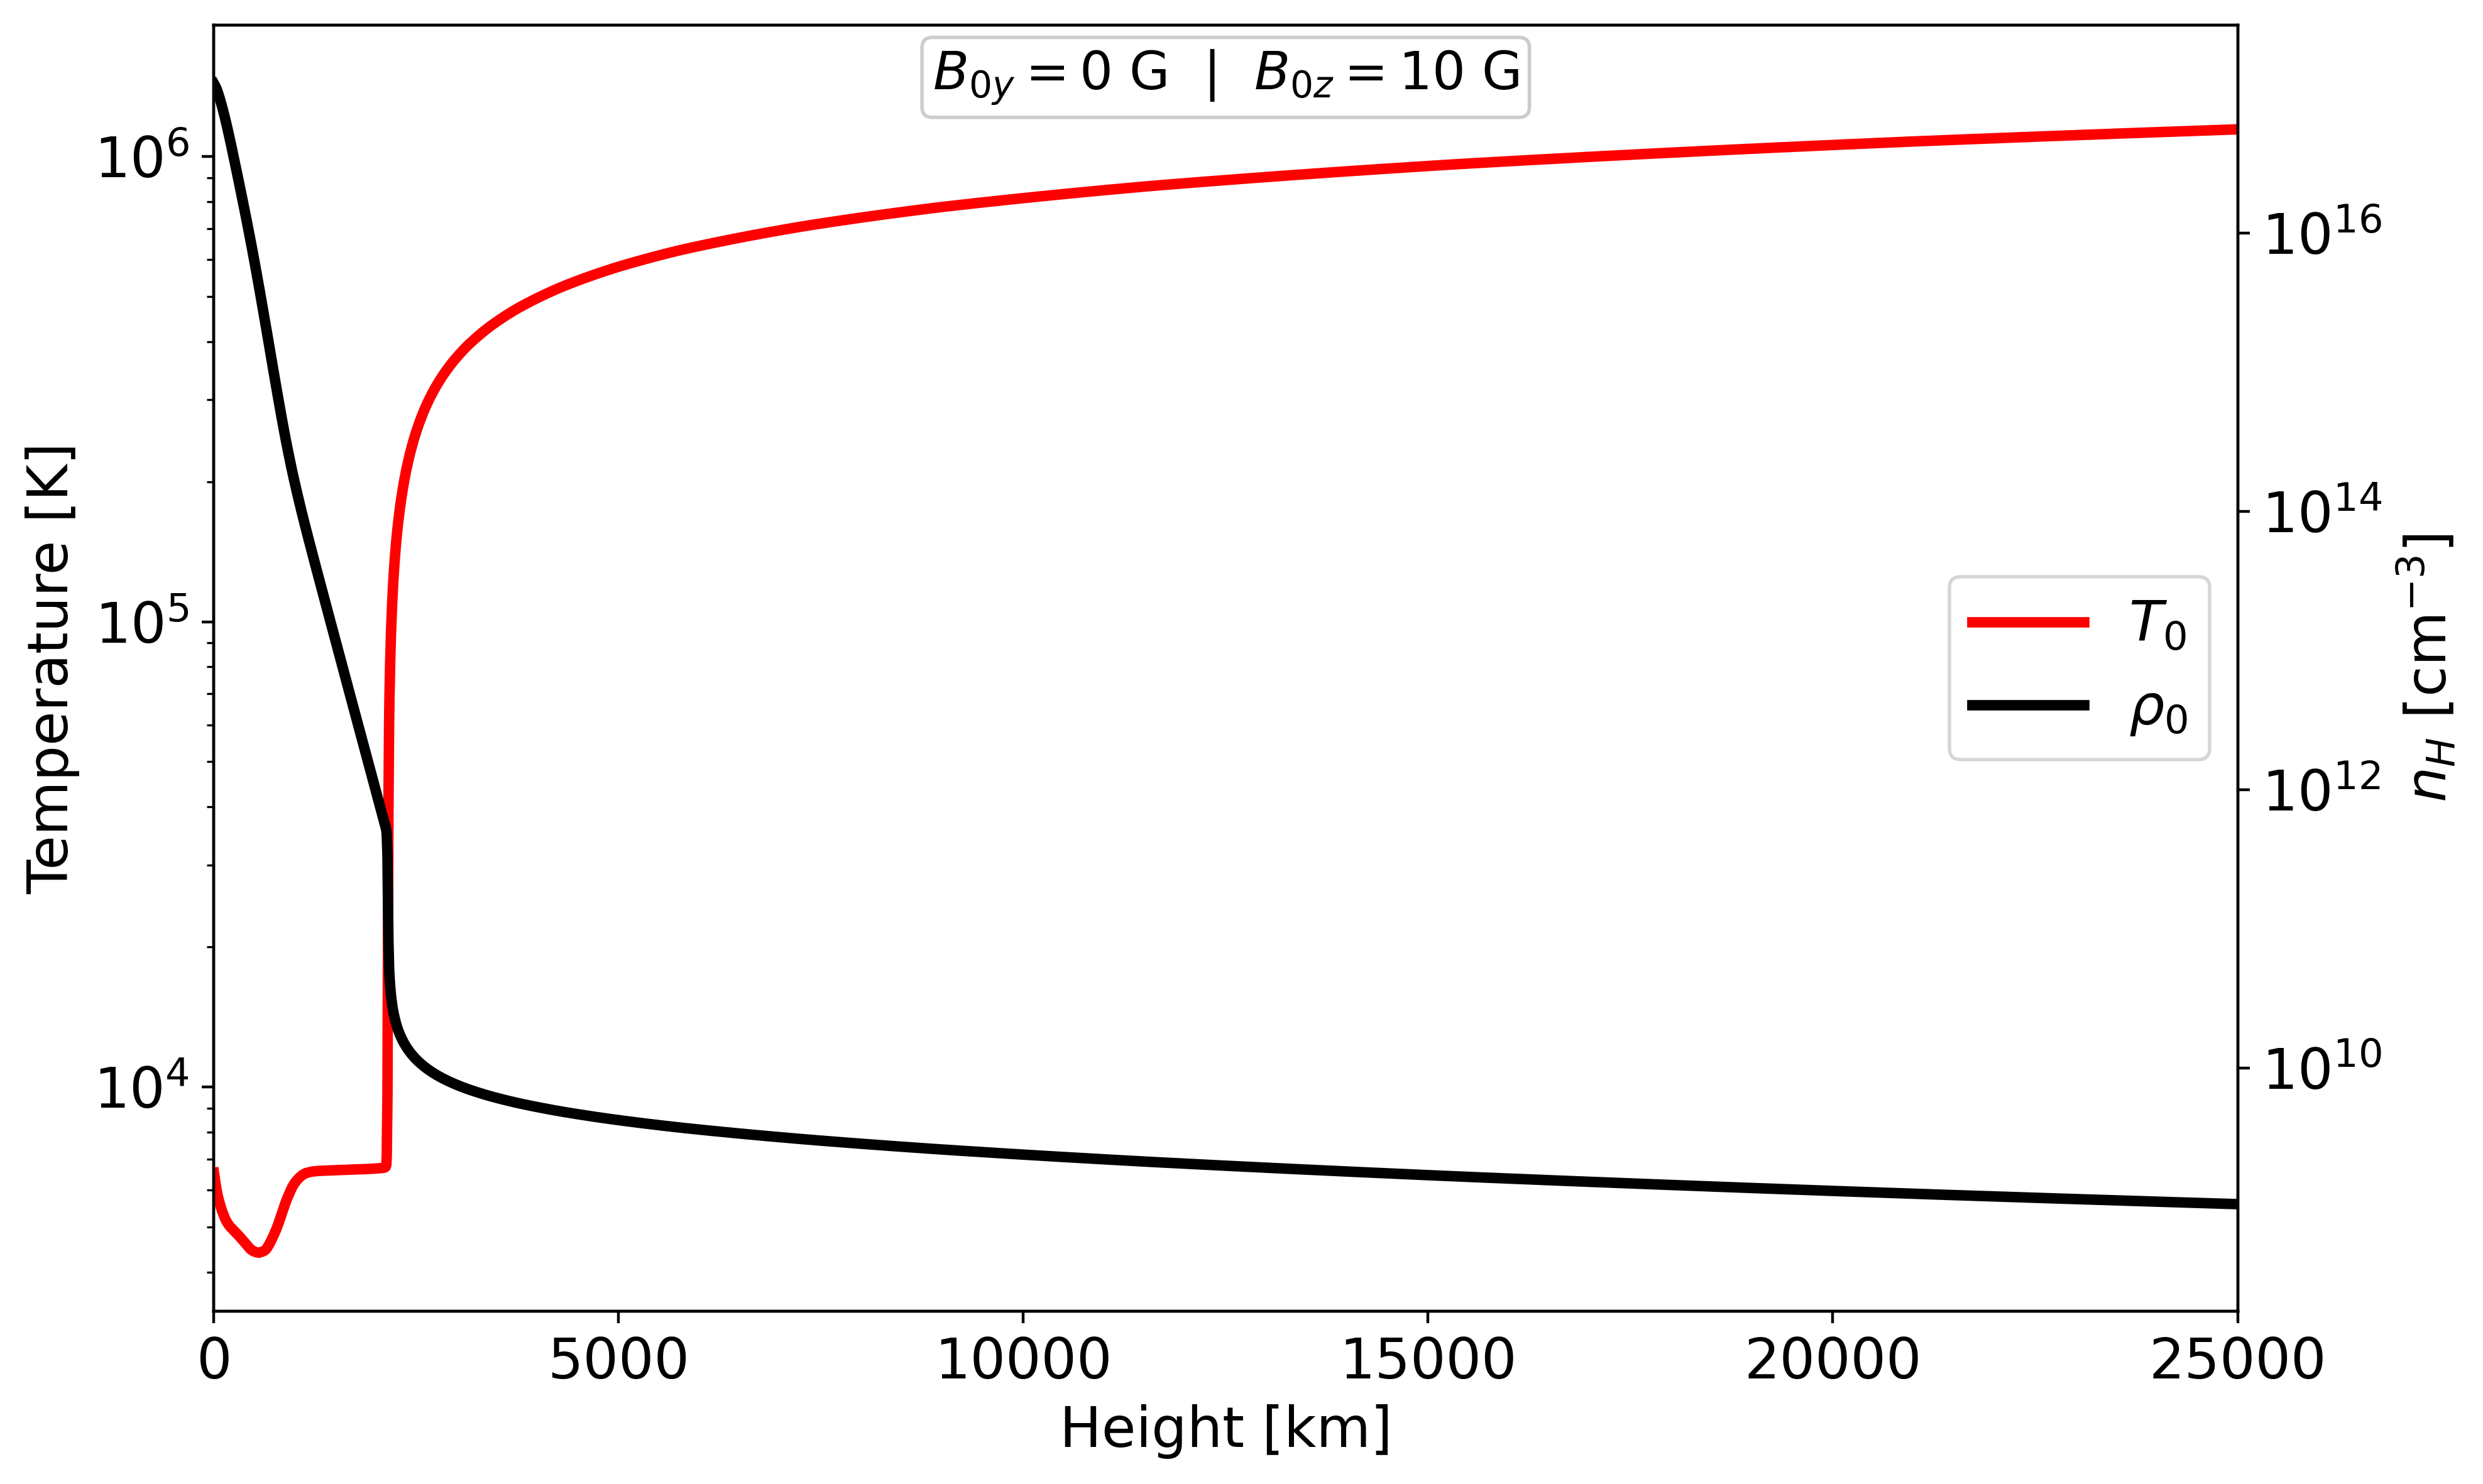
\includegraphics[width=0.8\textwidth]{profile.png}
  \caption{
    Equilibrium temperature profile (red) based on the solar atmospheric model by \citet{avrett2008}, with corresponding integrated density profile ($n_\text{H}$, black) from the ODE in Equation \eqref{eq: density_ode}. The magnetic field has a uniform $z$-component of 10G; the gravitational field is given by Equation
    \eqref{eq: solar_gravity}.
  }
  \label{fig: temperature-density-profile}
\end{figure}
The uniform magnetic field adopted implies that only the first term here enters, but one could allow for non-uniform, non force-free magnetic field variations by including this second term. The temperature derivative has to be done numerically and is calculated based on the high resolution interpolated profile using sixth order accurate finite difference methods, with forward and backward differences near the start and end of the grid, respectively, and central differences in between.


Equation \eqref{eq: density_ode} is then integrated for $\rho_0(x)$ using a fifth-order accurate Runge-Kutta method to obtain the density profile, which is then substituted back into the ODE in order to retrieve the density derivative. This approach in calculating the density derivative -- instead of numerically differentiating the obtained density profile -- satisfies the force-balance Equation \eqref{eq: simple_force_balance} as close as numerically possible. As unit normalisations we choose a reference temperature of 1 MK, magnetic field of 10 Gauss, and a unit length of 1000 km, which automatically constrains all other normalisations following the ideal gas law using a mean molecular weight of one. This results in a profile that corresponds to observational values of the solar atmosphere, as for example given by \citet{book_priest}. Figure \ref{fig: temperature-density-profile} shows the resulting temperature and density profiles as a function of height, extending up to 25 Mm above the solar surface, for a uniform magnetic field of 10 Gauss along the $z$-direction. These equilibria are subsequently passed on to {\legolas} with a given wave vector to calculate the spectra. Thermal conduction parallel to the magnetic field is included, together with optically thin radiative losses based on the {\spexdm} cooling curve by \citet{schure2009} as in Figure \ref{fig: coolingcurves}.


\subsection{Non-adiabatic continua} \label{ss: non_adiabatic_continua}
Before diving into the complex spectroscopy of a realistic solar atmosphere model, it is useful to have a first indication of stable and unstable configurations in order to locate possible parameter regions of interest. To that end we solve the continuum Equation \eqref{eq: slow_thermal_continuum} using the profiles discussed here for a range in wave numbers. Figure \ref{fig: continua_vsk} shows stability regions for both the thermal and slow continua over the entire temperature range shown in Figure \ref{fig: temperature-density-profile}, for a wave vector parallel to the magnetic field ($k_y = 0$) with $k_z$ varying between 0.05 and 10. The temperature profile is superimposed on both figures with a black line. Regions where the continua are unstable are coloured in green for the thermal continuum (Panel a) and in red for the slow continuum (Panel b). It can immediately be seen that the entire chromosphere up to the transition region at $\approx 2$ Mm has an unstable thermal continuum for the full range in wave number, and as soon as the lower corona is reached this becomes more and more stable, until only large-scale perturbations (small $k_z$) lead to unstable continuum regions. The high thermal instability of the solar chromosphere is mainly a consequence of the low temperature present there, which results in diminished parallel thermal conduction effects ($\sim T^{5/2}$) and hence less stability since temperature gradients are less efficiently smoothed out. The slow continuum on the other hand is completely stable in the chromosphere and is characterised by only a narrow unstable region in the lower corona. Panels c and d correspond to the horizontally dotted line at $k_z = 1$, and show the imaginary parts of the thermal (c) and slow (d) continua for that particular $k_z$-value as a function of height.

\begin{figure}[t]
  \centering
  \includegraphics[width=\textwidth]{{continua_SA_0-50_250pts_k3_0.05-10.0}.png}
  \caption{
    Panels \textbf{a} and \textbf{b}: stability regions of the thermal and slow continua for the temperature profile in Figure \ref{fig: temperature-density-profile}, for a range in $k_z$. Unstable regions are coloured in green and red for the thermal and slow continua, respectively. The black line denotes the temperature profile vs. height. Panels \textbf{c} and \textbf{d}: continuum solutions as a function of height for $k_z$ = 1, corresponding to the dotted line in Panels \textbf{a} and \textbf{b}.
  }
  \label{fig: continua_vsk}
\end{figure}

It should be noted that, in contrast to those for the analytic case in Figure \ref{fig: nye-thomas-continua}, the continua show sharp transitions and spiked behaviour, which is an unavoidable consequence of the cooling curve used. In the case of Figure \ref{fig: nye-thomas-continua} the continua are smooth because the equilibrium temperature was uniform, such that we only needed to evaluate the cooling curve and its derivatives in a single value. Here however we have a wide range in temperature, and while the heat-loss function $\HLFheat$ itself is continuous, the cooling curve has discontinuous derivatives since we do a local second-order approximation in between two data points (that is, between two ``original'' table values) in order to preserve the original table as closely as possible. As a consequence of this it is entirely possible that for some spatially varying temperature profiles there may be jumps in the continuum curves near temperature transitions between two table points. If one were to use a different representation for the cooling curve, that is, one that also has continuous derivatives $\dHLFrho$ and $\dHLFT$, this would yield smooth curves in the complex eigenvalue plane.

\begin{figure}[t]
  \centering
  \includegraphics[width=\textwidth]{{continua_SA_0-50_250pts_thetavary_k3_cost_k2_sint}.png}
  \caption{
    Panels \textbf{a} and \textbf{b}: stability regions of the thermal and slow continua for the temperature profile in Figure \ref{fig: temperature-density-profile}, for various angles between the wave vector $\bk$ and the magnetic field $\bb_0$. Unstable regions are coloured in green and red for the thermal and slow continua, respectively. Panels \textbf{c} and \textbf{d}: continuum solutions as a function of height for $\theta = 3\pi/8$, corresponding to the dotted line in Panels \textbf{a} and \textbf{b}.
  }
  \label{fig: continua_vstheta}
\end{figure}

Figure \ref{fig: continua_vstheta} keeps the magnitude of $k$ equal but varies the angle $\theta$ between the wave vector $\bk$ and the magnetic field $\bb_0$, hence $k_y = k_0\sin\theta$ and $k_z = k_0\cos\theta$. Stability regions for the thermal and slow continua are shown for $k_0 = 1$ and $\theta$ between 0 and $2\pi$, the case with $\theta = 0$ corresponds to the dotted line case at $k_z = 1$ in Figure \ref{fig: continua_vsk}. As the wave vector becomes more perpendicular to the magnetic field, the thermal continuum becomes more and more unstable, due to the fact that parallel thermal conduction is less efficient for larger angles. For near-perpendicular propagation the thermal continuum is unstable over the entire domain, owing to the almost complete loss of stability provided by parallel conduction. The slow continuum is mostly stable, with a few unstable regions similar to the previous case. In this Figure \ref{fig: continua_vstheta}, Panels c and d show the continua as a function of height, corresponding to the dotted horizontal line at $\theta = 3\pi/8$. We conclude that in the framework of single-fluid MHD adopted here, the entire chromosphere to corona of our realistic model is found liable to thermal instability, while the lower coronal regions in addition demonstrate slow continuum overstabilities, with corresponding travelling, singular modes at altitudes between $\approx 2.5 -- 8$ Mm.



\subsection{MHD spectra for the solar corona} \label{ss: corona_spectra}
\subsection{MHD spectra for the solar chromosphere} \label{ss: chromosphere_spectra}

\section{Discussion}



\cleardoublepage
